\documentclass[10pt,letterpaper,bibliography=totoc]{scrartcl}

\usepackage[letterpaper,margin=1.2in]{geometry}
\usepackage{helvet}
\usepackage{graphicx}
\usepackage[hyphens]{url}
\usepackage{hyperref}
\usepackage[all]{hypcap} 
\usepackage{xcolor}
\usepackage{listings}
\usepackage[T1]{fontenc}
\usepackage{verbatim}
\usepackage[parfill]{parskip}

\lstset{
    basicstyle=\scriptsize,
    numbers=left,
    numberstyle=\scriptsize,
    stepnumber=1,
    numbersep=5pt,
    showspaces=false,
    showstringspaces=false,
    showtabs=false,
    frame=shadowbox,
    tabsize=4,
    captionpos=b,
    breaklines=true,
    breakatwhitespace=false,
    keywordstyle=\color{blue!70},
    commentstyle=\color{red!50!green!50!blue!50},
    rulesepcolor=\color{red!20!green!20!blue!20},
    numberbychapter=false,
    stringstyle=\ttfamily
}

\setcounter{tocdepth}{2}

\hypersetup{
    colorlinks=true,
    breaklinks=true,
    urlcolor=blue,
    linkcolor=black
}

\begin{document}

\author{Orkun Krand}
\title{Assignment 2}
\subtitle{Fall 2017\\ CS834 Introduction to Information Retrieval\\ Dr. Michael Nelson}
\maketitle
\newpage

\section{Question 4.1}
\subsection {Question}
Plot rank-frequency curves (using a log-log graph) for words and bigrams in the Wikipedia collection available through the book website ( http://www.search-engines-book.com ). Plot a curve for the combination of the two. What are the best values for the parameter c for each curve?

\subsection{Methodology}
I wrote a Python script \texttt{pagevisitor.py} that uses \href{www.nltk.org}{NLTK} (Natural Language Toolkit) and \href{https://www.crummy.com/software/BeautifulSoup/}{BeautifulSoup} to access a folder and its subfolders (looking for 'en' as default as it is the root folder of the Wikipedia corpus from the book website), and process the documents found to collect word, bigram, and inlink information. By the time I realized I should've converted everything to lowercase to avoid duplicates, it was too late. \texttt{q1graphs.r} was created to visualize the data collected by \texttt{pagevisitor.py}

\subsection{Results}
\texttt{pagevisitor.py} found 232,919 words and 1,662,253 bigrams. Visualizing these numbers, we receive the following graphs: 

\begin{figure}[!h]
\centering
\label{fig:wordcount}
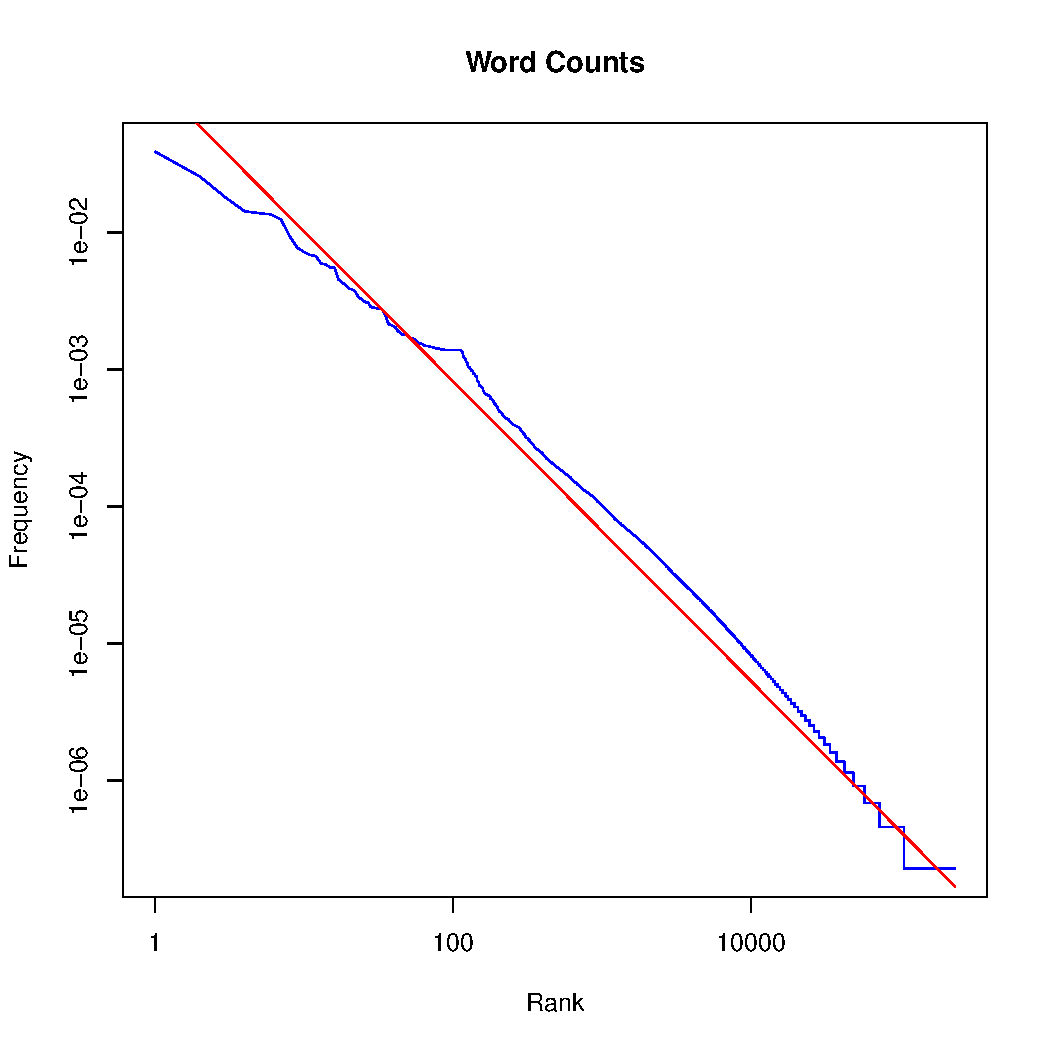
\includegraphics[scale=.5]{wordcount.pdf}
\caption{Word Count}
\end{figure}

Maximum likelihood estimation of words

Call:
mle(minuslogl = ll, start = list(s = 1))

Coefficients:
  Estimate   Std. Error
s 1.002823 0.0001287333

-2 log L: 73354417 

C = 1.269302e-01

\hfill \linebreak
\begin{figure}[!h]
\centering
\label{fig:bigram}
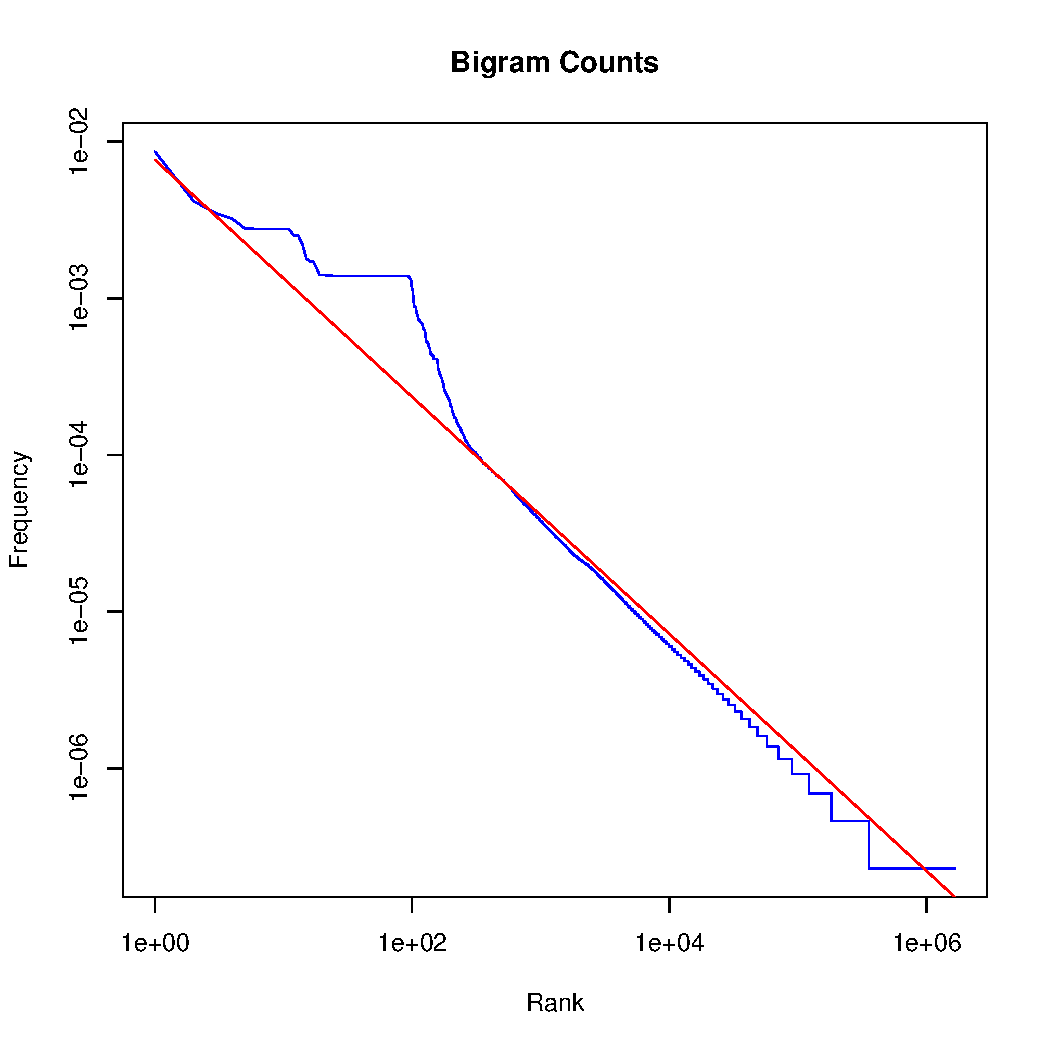
\includegraphics[scale=.5]{bigram.pdf}
\caption{Bigram Count}
\end{figure}

Maximum likelihood estimation of bigrams

Call:
mle(minuslogl = ll, start = list(s = 1))

Coefficients:
   Estimate   Std. Error
s 0.8292686 0.0001292527

-2 log L: 106198894 

C = 7.650163e-03

\hfill \linebreak
\begin{figure}[!h]
\centering
\clearpage
\label{fig:both}
\includegraphics[scale=.5]{word_bigram.pdf}
\caption{Both Word and Bigram Counts }
\end{figure}

Maximum likelihood estimation of combined

Call:
mle(minuslogl = ll, start = list(s = 1))

Coefficients:
   Estimate   Std. Error
s 0.9250651 8.066917e-05

-2 log L: 191232526 

C = 3.019035e-02

\hfill \linebreak
\section{Question 4.2}
\subsection {Question}
Plot vocabulary growth for the Wikipedia collection and estimate the parameters for Heaps' law. Should the order in which the documents are processed make any difference?

\subsection{Methodology}
Modifying \texttt{pagevisitor.py} to keep track of vocabulary (unique words) and total words and logging them after accessing each document enabled me to create the required plot for this question. Using \texttt{q2graphs.r}, I was able to create visualizations. 

\subsection{Results}
\begin{figure}[h!]
\centering
\label{fig:vocab}
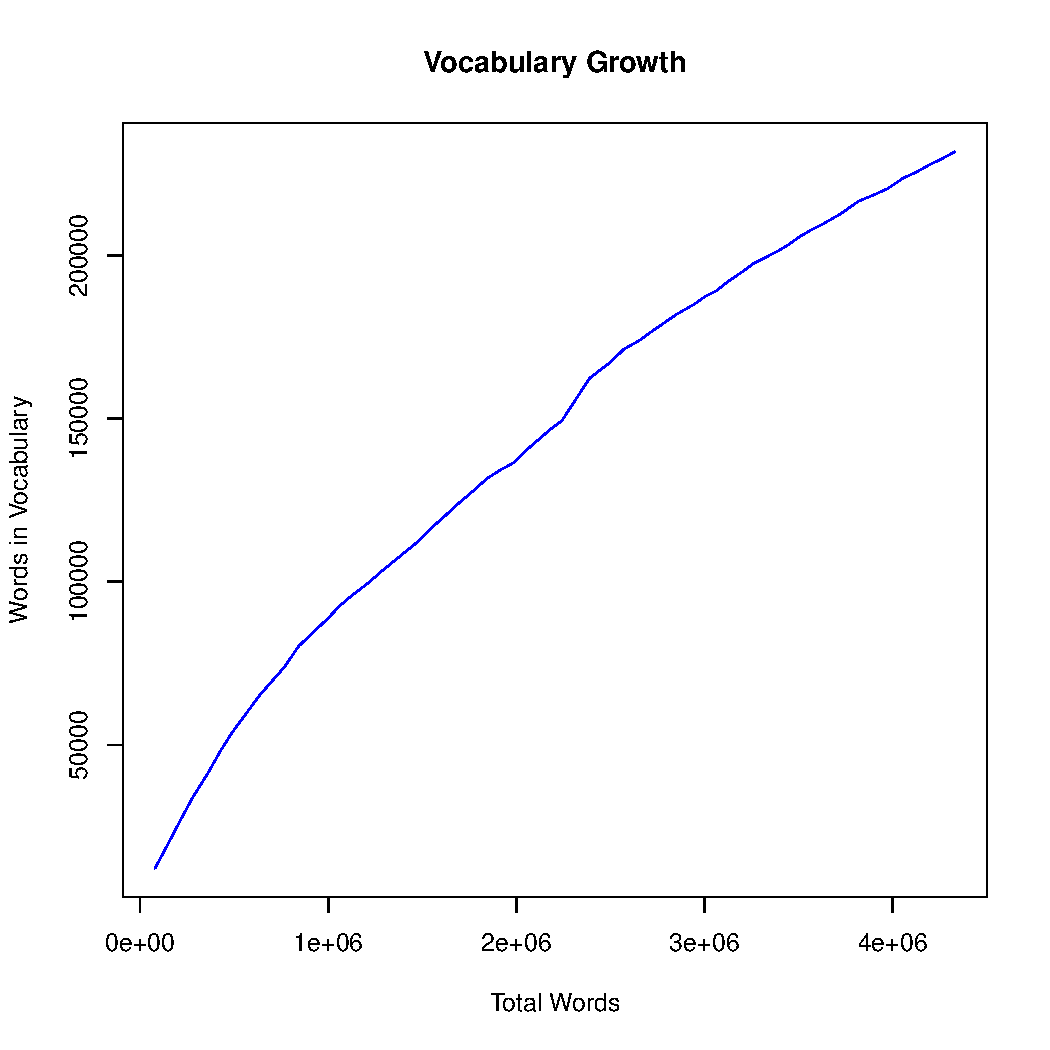
\includegraphics[scale=.5]{vocabulary.pdf}
\caption{Vocabulary Growth}
\end{figure}

The order in which the documents are processed is important for Heap's Law because we compute the sum of all words in the dictionary after processing each document. 
\clearpage

\section{Question 4.3}
\subsection {Question}
Try to estimate the number of web pages indexed by two different search engines
using the technique described in this chapter. Compare the size estimates
from a range of queries and discuss the consistency (or lack of it) of these estimates.

\subsection{Methodology}
According to the book\cite{classtext}, assuming the two terms are independent of each other,

\begin{equation}\label{eq:numindexedpages1}
  f_{ab} = N \cdot f_a/N \cdot f_b/N
\end{equation}

\begin{equation}\label{eq:numindexedpages2}
    N = (f_{a} \cdot f_{b}) / f_{ab}
\end{equation}

I will use \href{www.google.com}{Google} and \href{www.yahoo.com}{Yahoo!} for this assignment. The queries I will use are ``motorcycle cake'' and ``yamaha quinoa''. 

\subsection {Results}
Working with Google first:
\begin{figure}[h!]
\centering
\label{fig:motorcycleGoogle}
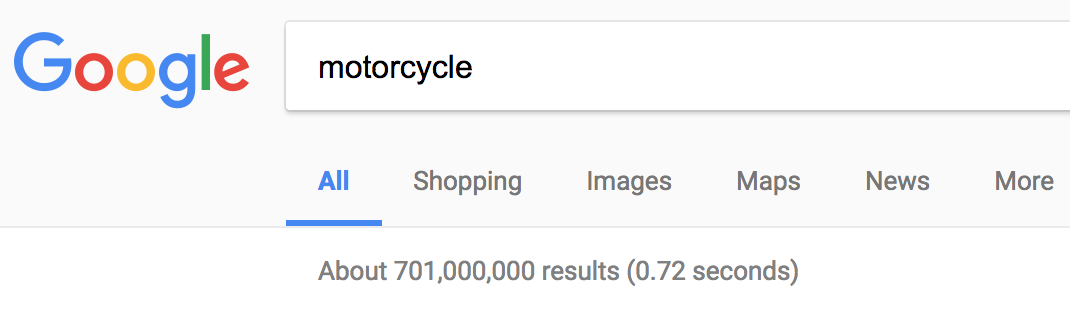
\includegraphics[scale=.5]{motorcycle_google.png}
\caption{Google: motorcycle}
\end{figure}
\begin{figure}[h!]
\centering
\label{fig:cakeGoogle}

\includegraphics[scale=.5]{cake_google.png}
\caption{Google: cake}
\end{figure}
\begin{figure}[h!]
\centering
\label{fig:motorcycleCakeGoogle}

\includegraphics[scale=.5]{motorcycle-cake_google.png}
\caption{Google: motorcycle cake}
\end{figure}
\begin{figure}[h!]
\centering
\label{fig:yamahaGoogle}
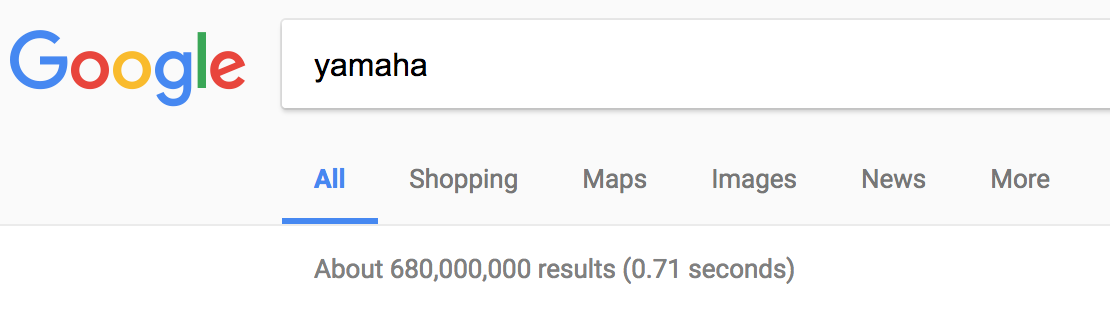
\includegraphics[scale=.5]{yamaha_google.png}
\caption{Google: yamaha}
\end{figure}
\begin{figure}[h!]
\centering
\label{fig:quinoaGoogle}
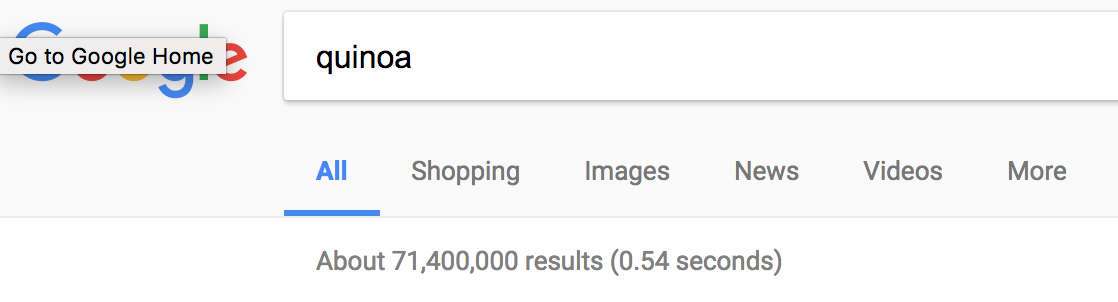
\includegraphics[scale=.5]{quinoa_google.png}
\caption{Google: quinoa}
\end{figure}
\begin{figure}[h!]
\centering
\label{fig:yamahaQuinoaGoogle}

\includegraphics[scale=.5]{yamaha-quinoa_google.png}
\caption{Google: yamaha quinoa}
\end{figure}
\hfill \linebreak

According to the first query, the size of Google is:
\begin{equation}\label{eq:GoogleSize1}
    N = \frac{(701,000,000 \cdot 969,000,000)}{18,100,000} = 37,528,674,033
\end{equation}

The second query, using the equation in the book gives us:
\begin{equation}\label{eq:GoogleSize2}
    N = \frac{(680,000,000 \cdot 71,400,000)}{276,000} = 175,913,043,478
\end{equation}

These two numbers are very far away from each other. This may be due to \textit{motorcycle} and \textit{cake} both being generic terms whereas \textit{yamaha} and \textit{quinoa} are more specific terms that are not related. So if I had to pick between these two results, I would pick the larger (176B) as the better estimation for the size of Google.

Let's do the same for Yahoo!:
\begin{figure}
\centering
\label{fig:motorcycleYahoo}
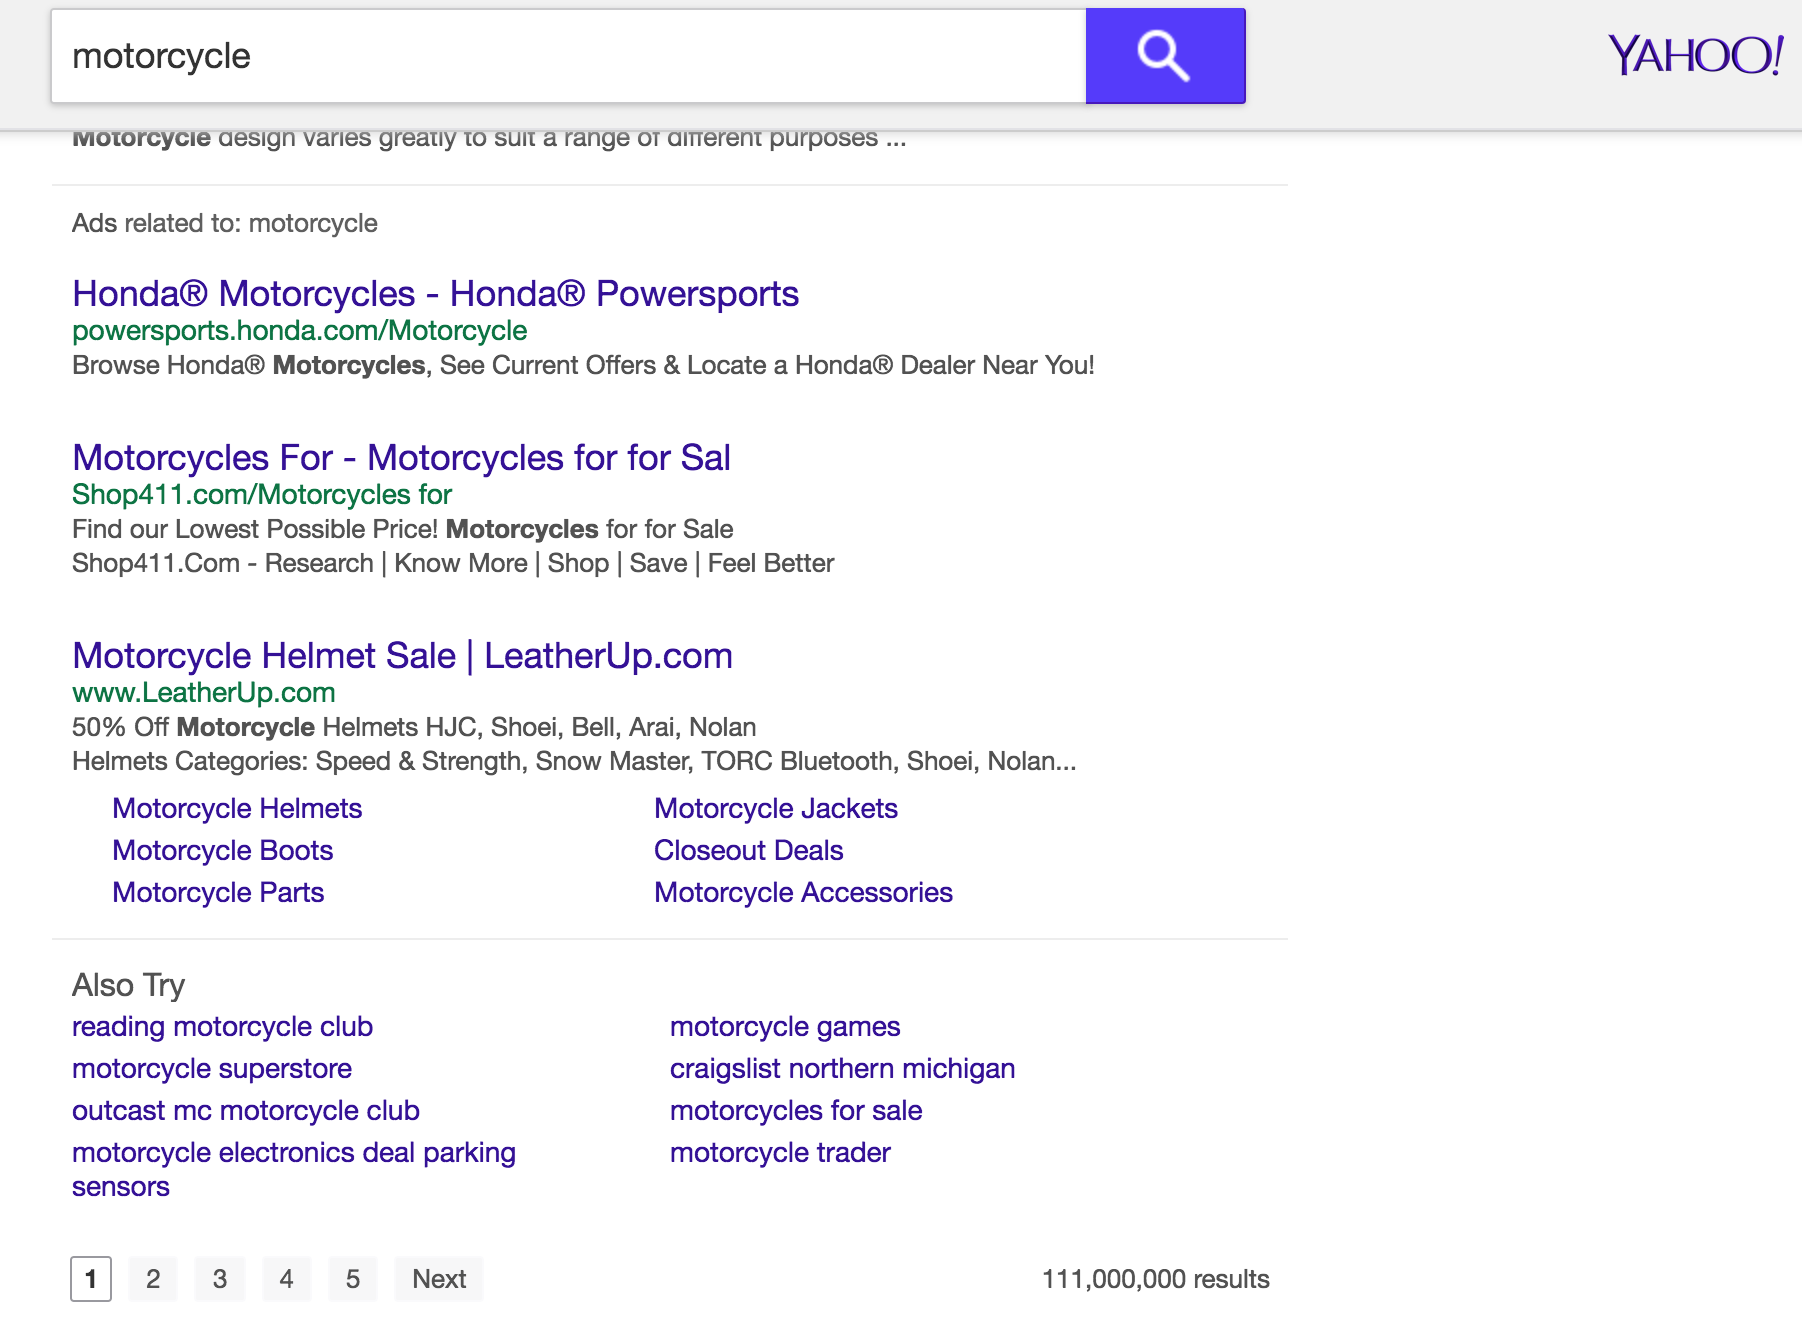
\includegraphics[scale=.3]{motorcycle_yahoo.png}
\caption{Yahoo: motorcycle}
\end{figure}
\begin{figure}
\centering
\label{fig:cakeYahoo}
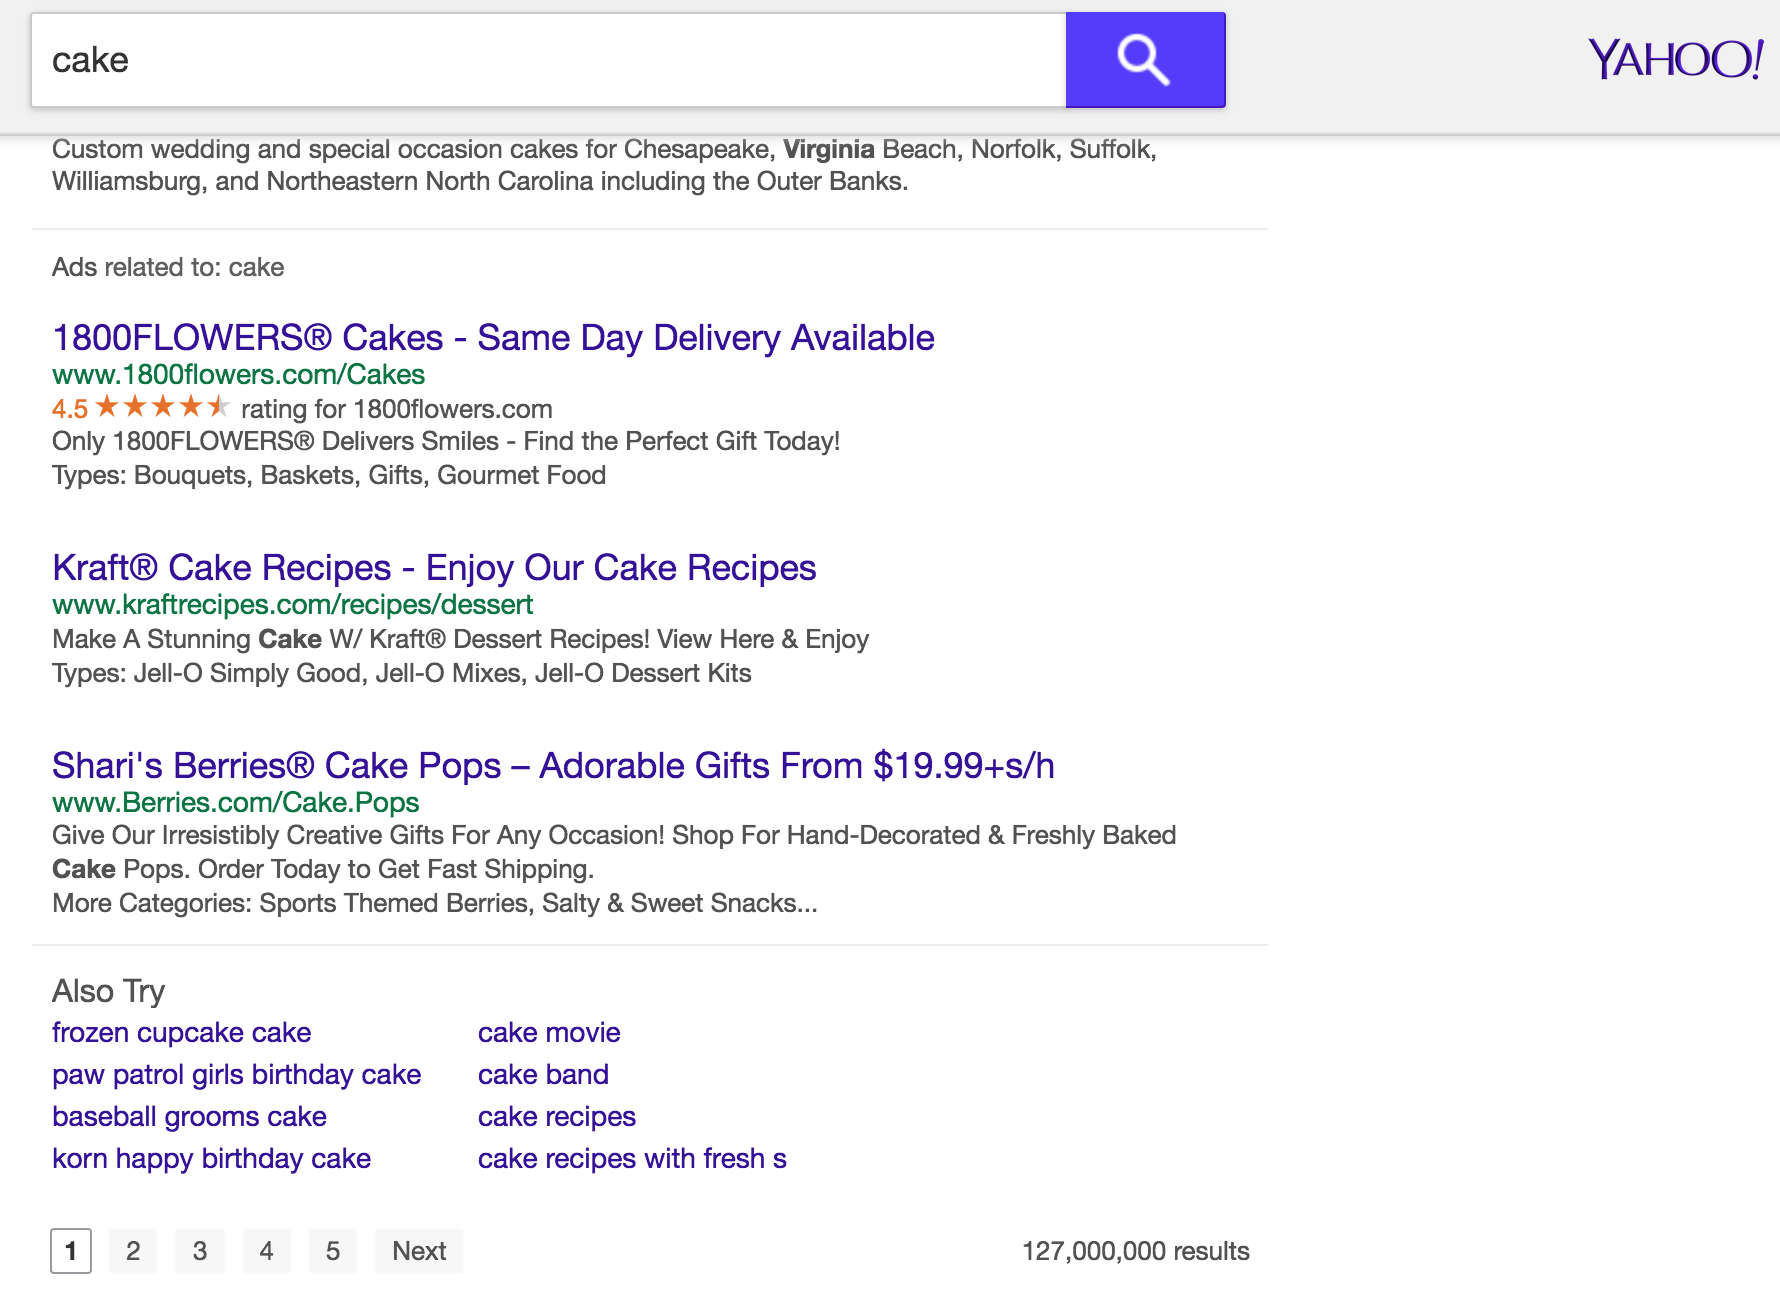
\includegraphics[scale=.3]{cake_yahoo.png}
\caption{Yahoo: cake}
\end{figure}
\begin{figure}
\centering
\label{fig:motorcycleCakeYahoo}
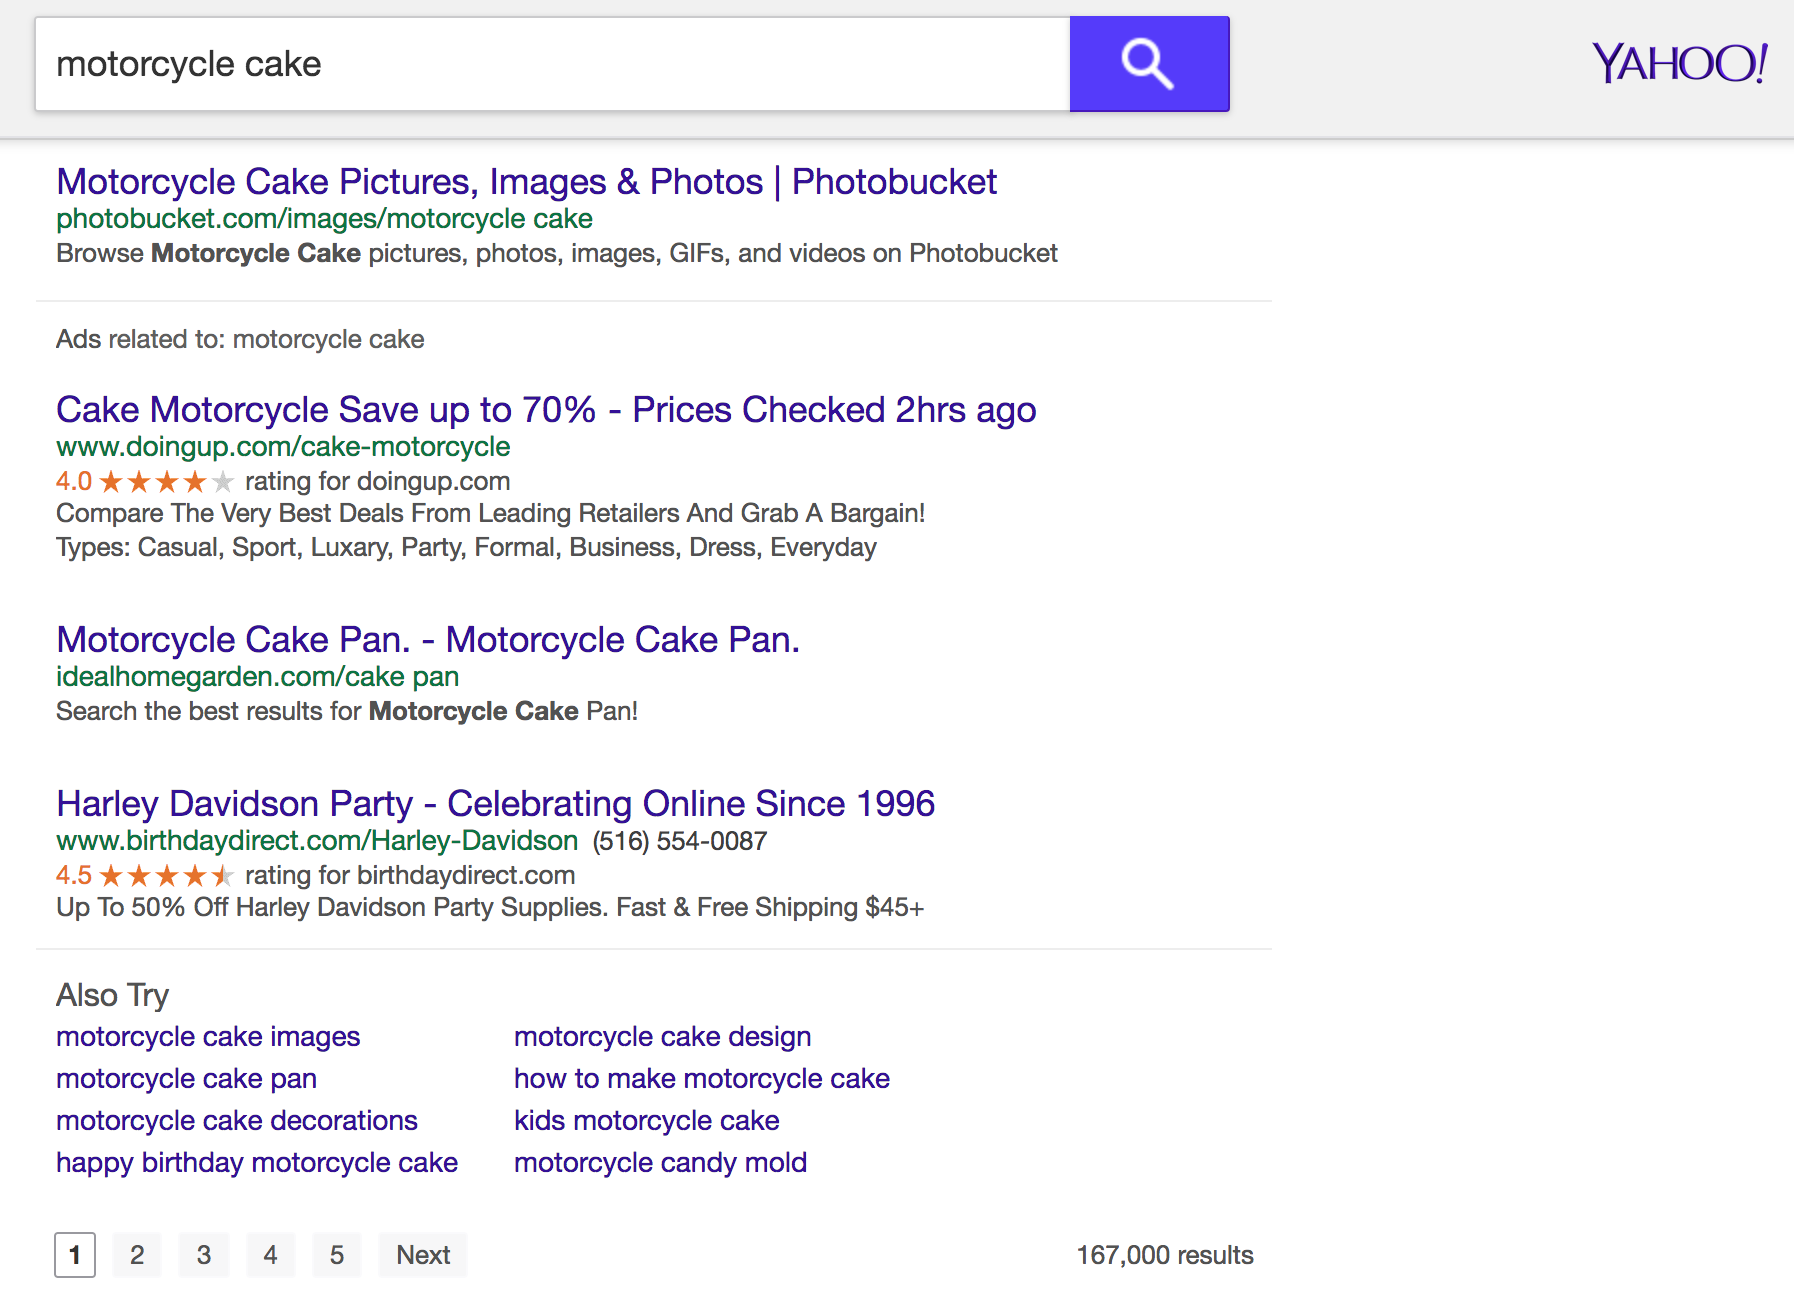
\includegraphics[scale=.3]{motorcycle-cake_yahoo.png}
\caption{Yahoo: motorcycle cake}
\end{figure}
\begin{figure}
\centering
\label{fig:yamahaYahoo}
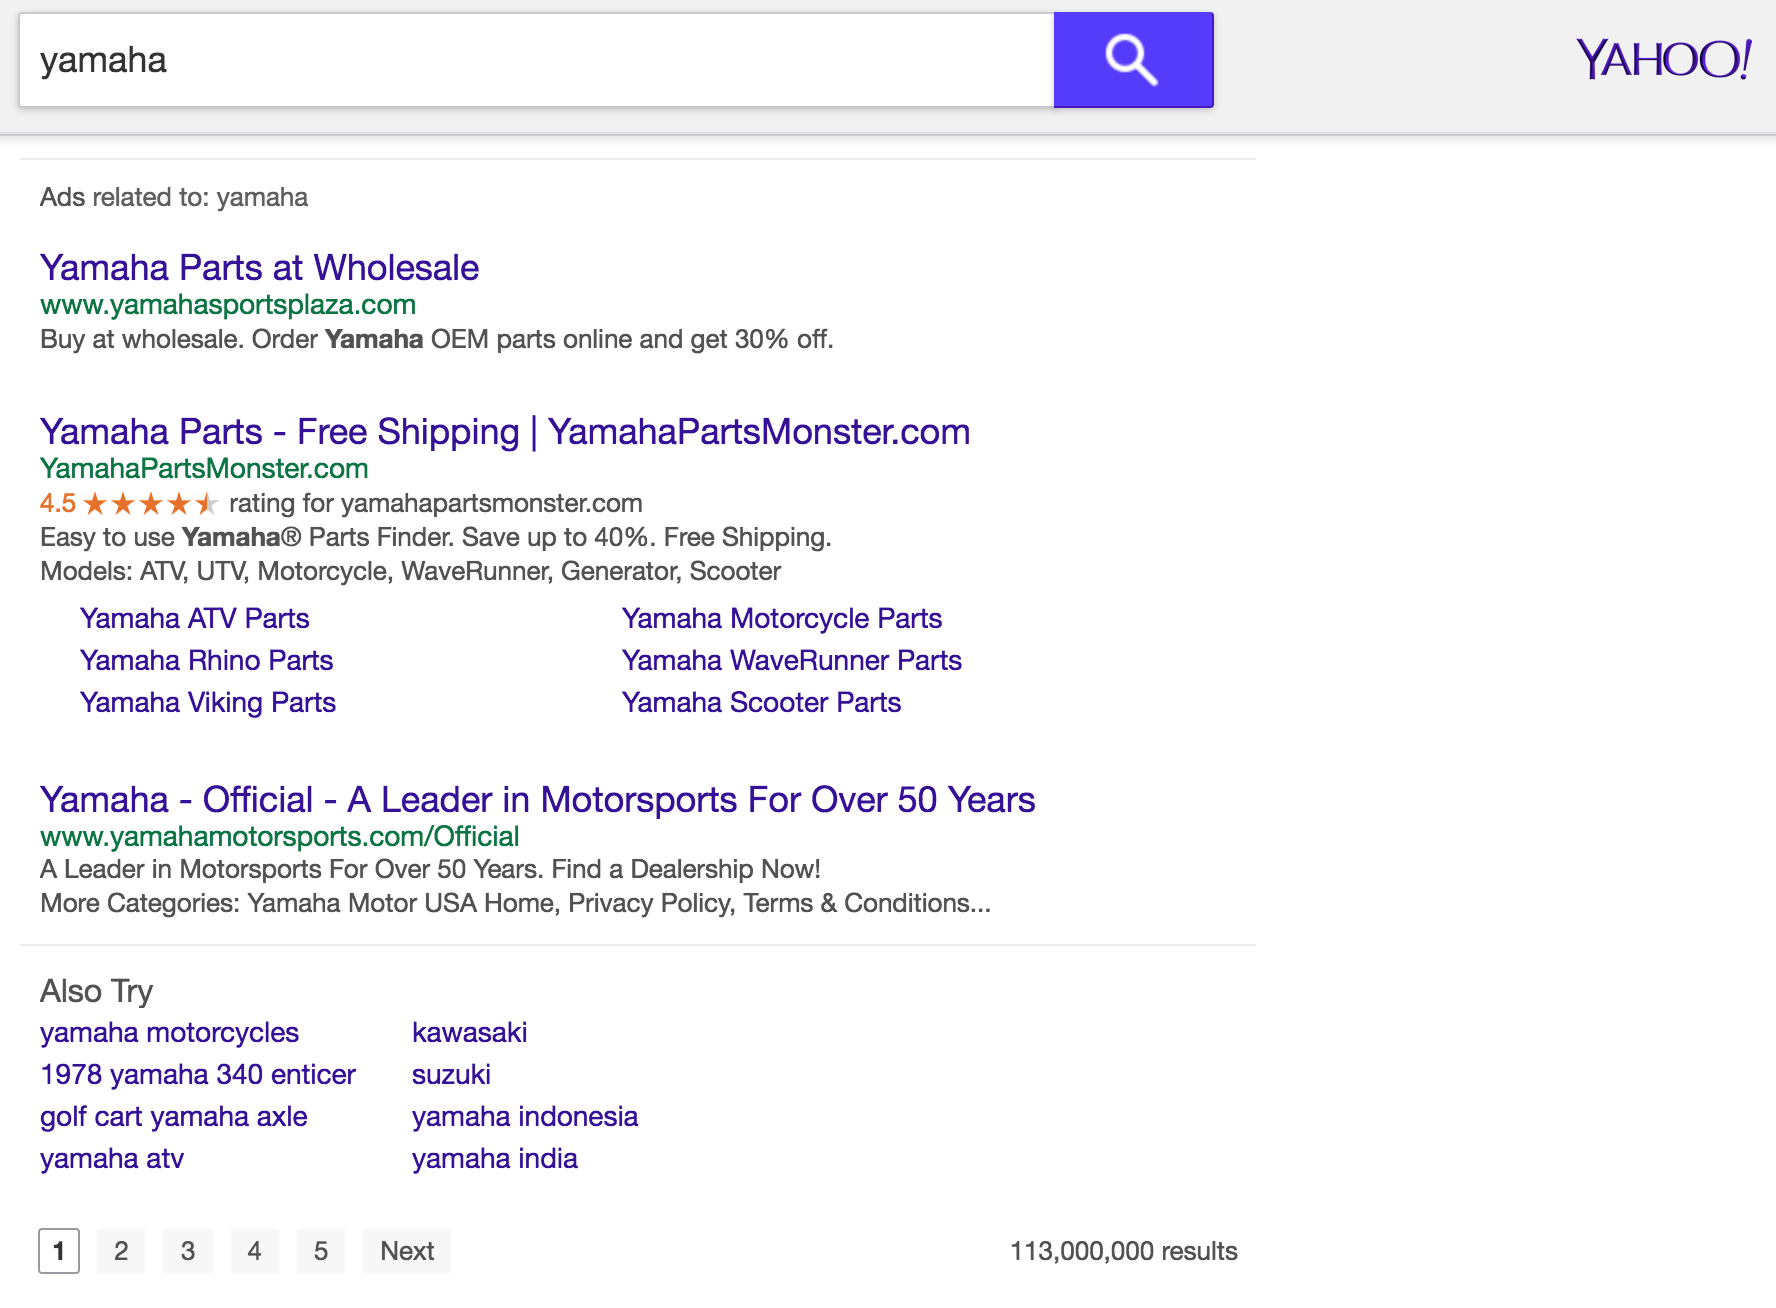
\includegraphics[scale=.3]{yamaha_yahoo.png}
\caption{Yahoo: yamaha}
\end{figure}
\begin{figure}
\centering
\label{fig:quinoaYahoo}
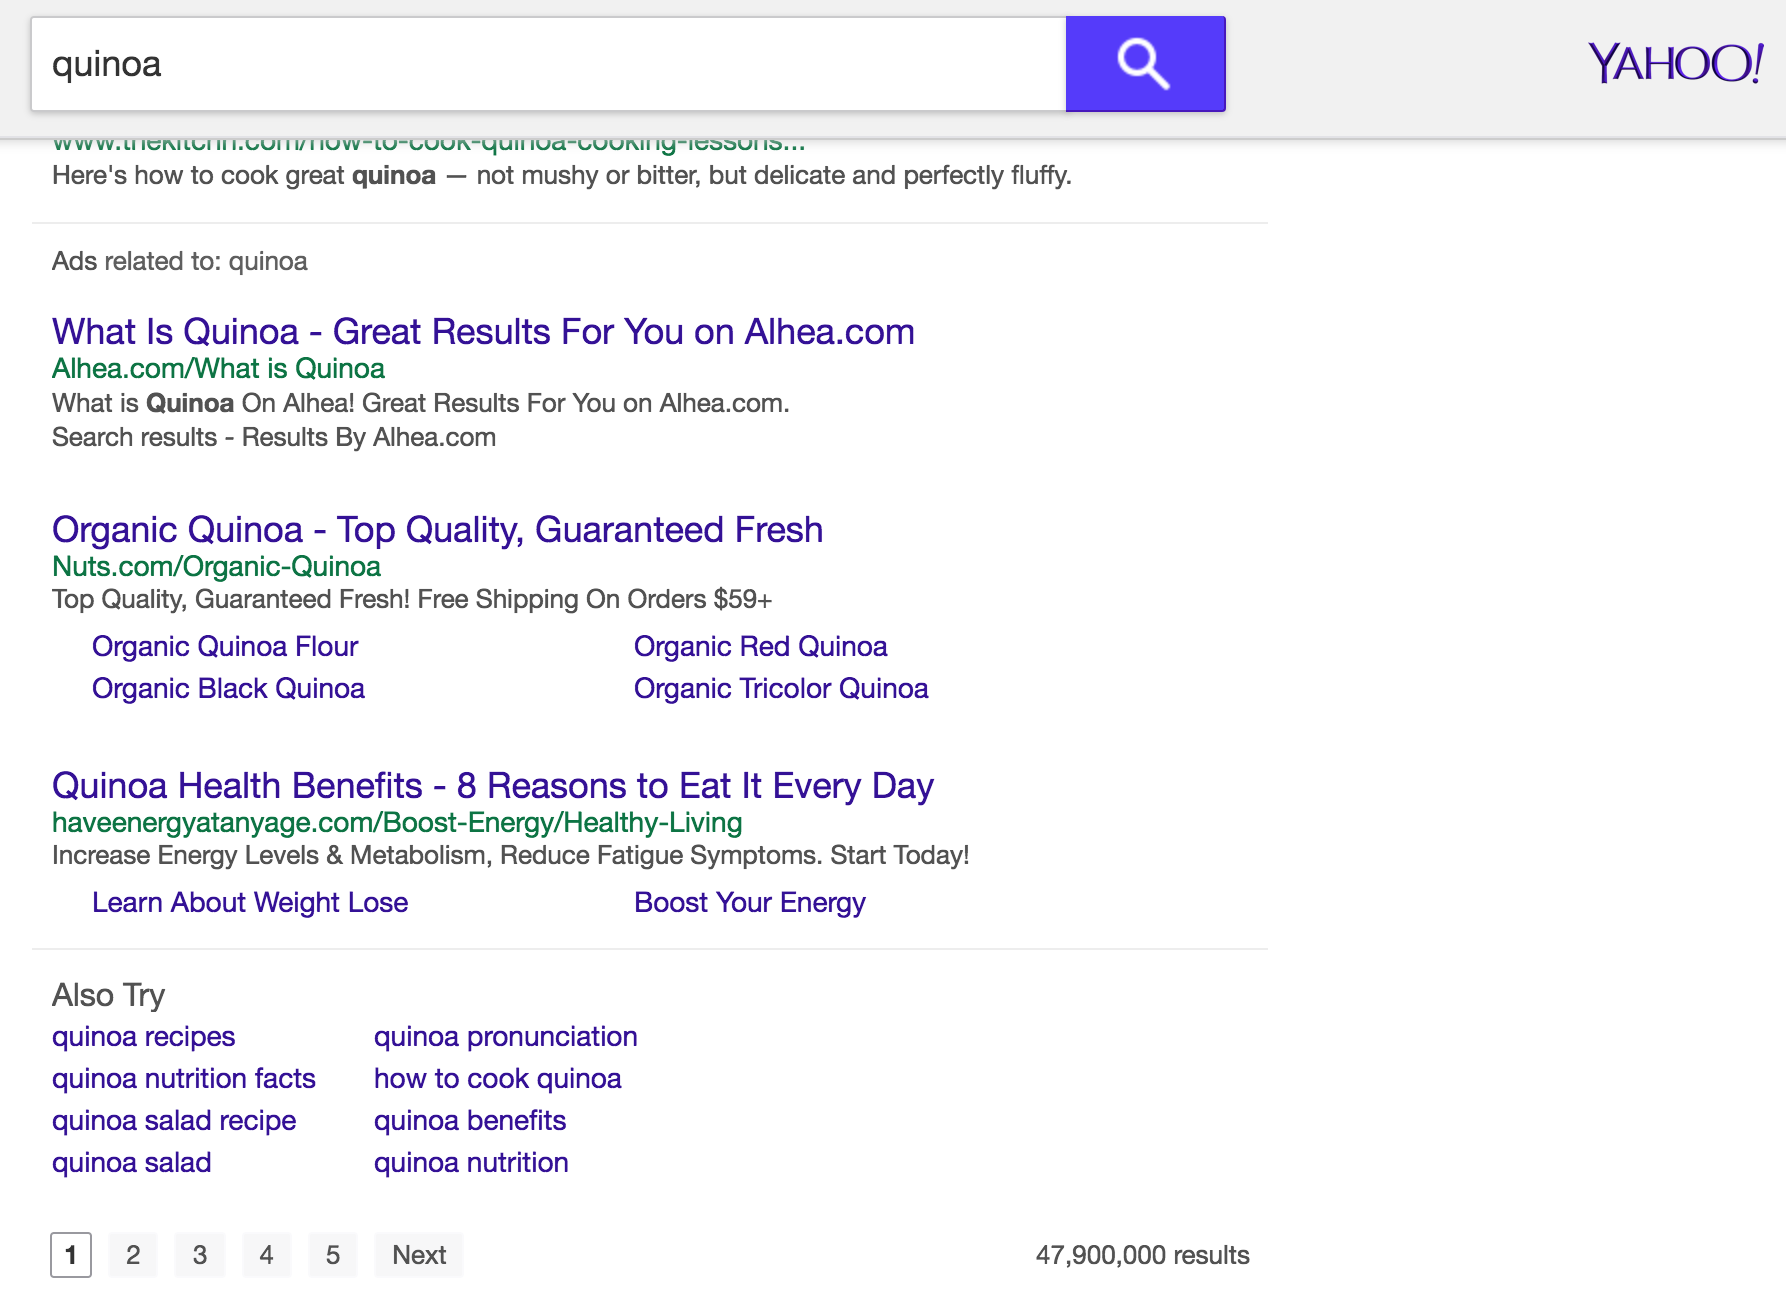
\includegraphics[scale=.3]{quinoa_yahoo.png}
\caption{Yahoo: quinoa}
\end{figure}
\begin{figure}
\centering
\label{fig:yamahaQuinoaYahoo}
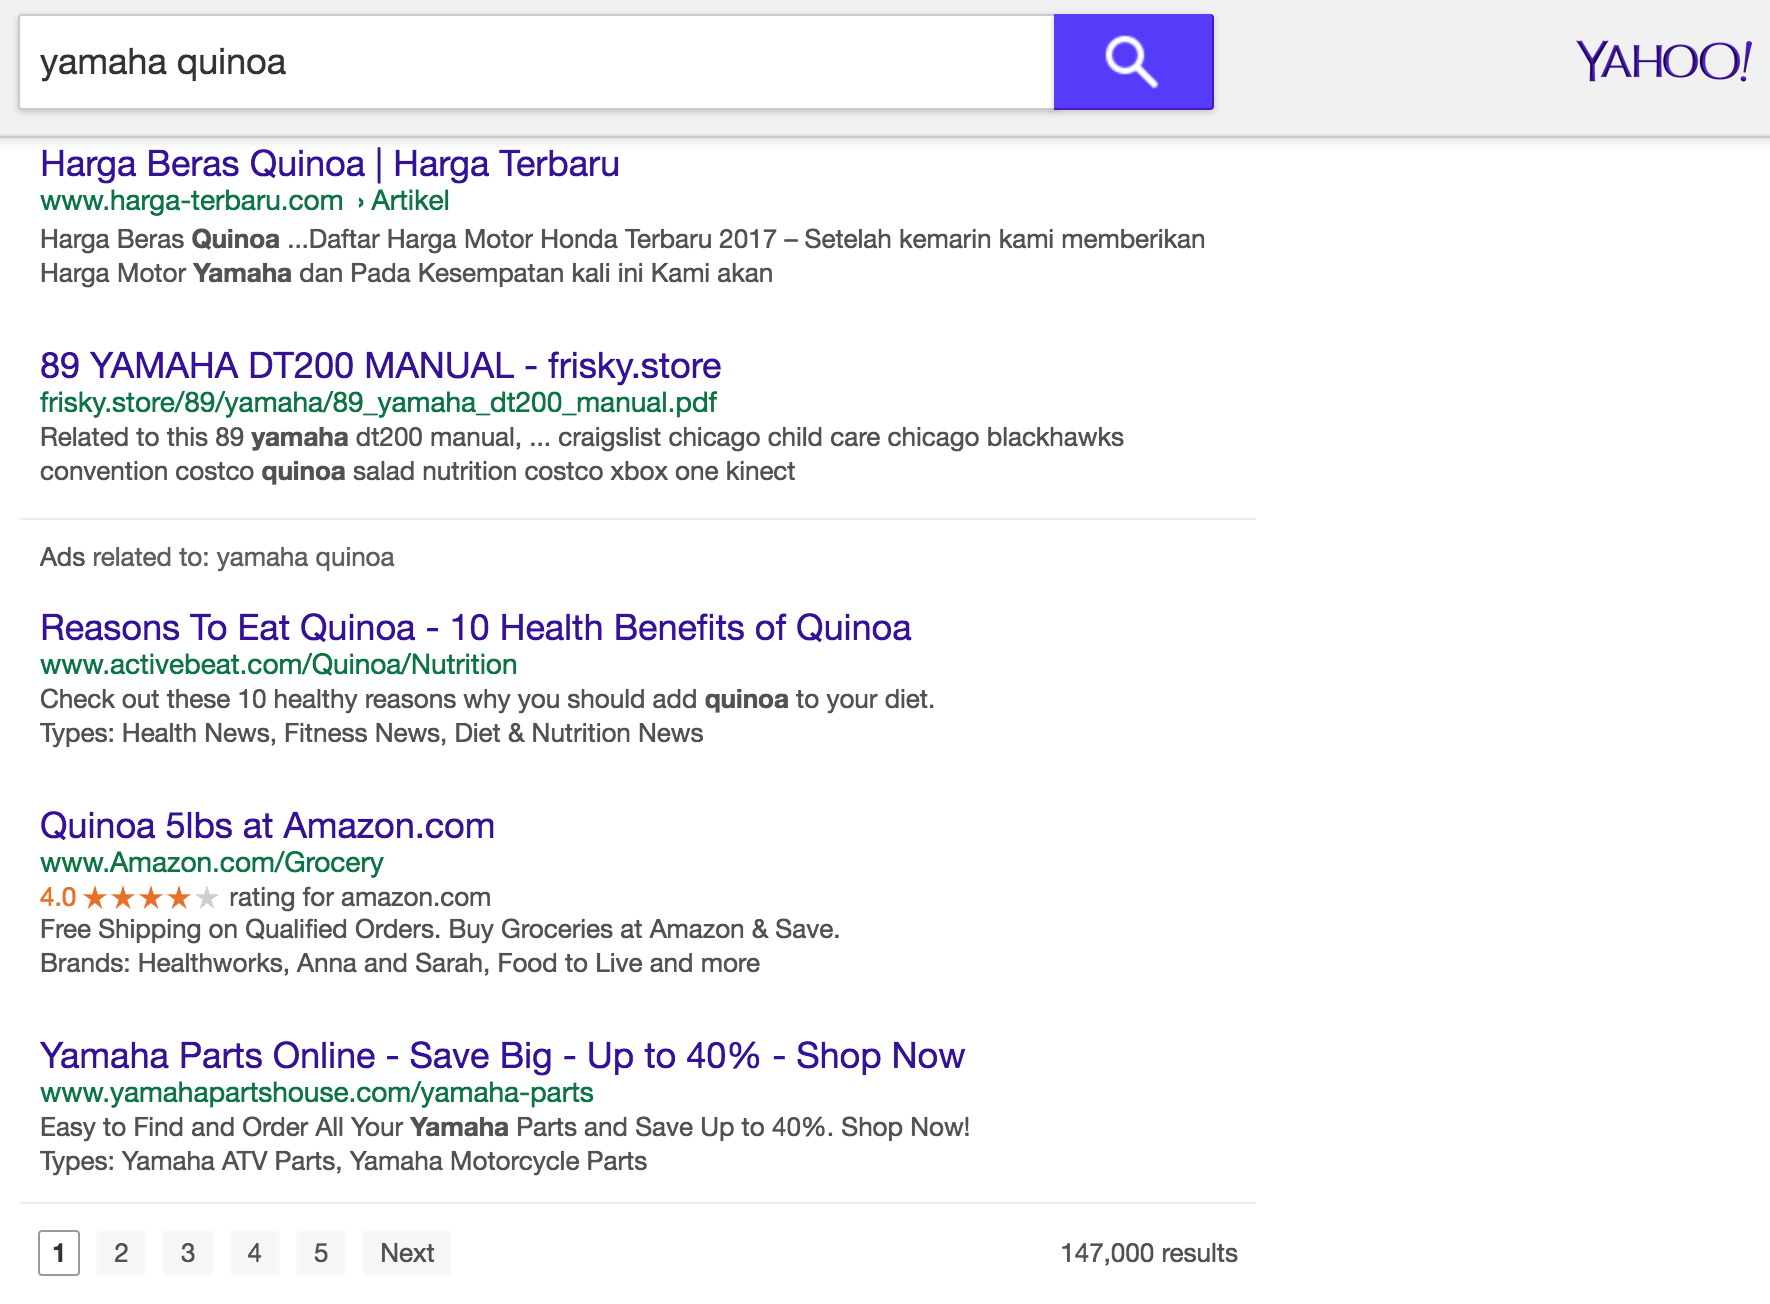
\includegraphics[scale=.3]{yamaha-quinoa_yahoo.png}
\caption{Yahoo: yamaha quinoa}
\end{figure}

According to the first query, the size of Yahoo! is:
\begin{equation}\label{eq:YahooSize1}
    N = \frac{(111,000,000 \cdot 127,000,000)}{167,000} = 84,413,173,652
\end{equation}

The second query, using the equation in the book gives us:
\begin{equation}\label{eq:YahooSize2}
    N = \frac{(113,000,000 \cdot 47,900,000)}{147,000} = 36,821,088,435
\end{equation}

Unlike the first case, the second equation gave a smaller number than the first. But I still find the second number more believable because of the reason I explained earlier. This would mean that Google is almost 5 times bigger than Yahoo!. Checking out the real numbers surely would be interesting. 

\section{Question 4.8}
\subsection {Question}
Find the 10 Wikipedia documents with the most inlinks. Show the collection of anchor text for those pages.

\subsection{Methodology}
Modifying \texttt{pagevisitor.py} to find the inlinks for every page accessed was required for to find the top 10. Anchor text was also added to the output. Sorting them based on the number of inlinks gave me the top 10 pages. 

\subsection{Results}

\begin{table}
\begin{center}
  \begin{tabular}{ | l | r | r | }
    \hline
    Number of Inlinks & URI & Anchor Text \\
    \hline
    2264 & articles/2/0/0/2007.html & 2007, As of 2007 \\
    1896 & articles/s/m/a/User\%7ESmackBot\_cc7a.html & SmackBot \\
    1770 & articles/2/0/0/2008.html & 2008 \\
    1363 & articles/u/n/i/United\_States\_09d4.html & United States Of America, \\
     & & USA, Union, Thirteen Colonies, U.S., \\
     & & United States of America, US, \\
     & & United States, American, \\
     & & Americans, America, \\
     & & American nation, American citizen \\
    982 & articles/2/0/0/2006.html & 2006 \\
    791 & articles/a/l/a/User\%7EAlaibot\_de3d.html & Alaibot \\
    676 & articles/c/y/d/User\%7ECydebot\_38a6.html & Cydebot \\
    675 & articles/l/i/v/Category\%7ELiving\_people\_7259.html & Living people \\
    663 & articles/b/l/u/User\%7EBluebot\_e595.html & Bluebot \\
    655 & articles/g/e/o/Geographic\_coordinate\_system.html & coordinates, Location, Coordinates \\
    \hline
  \end{tabular}
\caption{Top Ten Pages With the Highest Number of Inlinks}
\label{table:inlinks}
\end{center}
\end{table}
\clearpage

\section{Question 5.8}
\subsection{Question}
Write a program that can build a simple inverted index of a set of text documents. Each inverted list will contain the file names of the documents that contain that word.
Suppose the file A contains the text ``the quick brown fox'', and file B contains ``the slow blue fox''. 

\begin{verbatim}
The output of your program would be:
% ./your-program A B
blue B
brown A
fox A B
quick A
slow B
the A B
\end{verbatim}

\subsection{Methodology}
Modifying the \texttt{pagevisitor.py} script allowed me to create an inverted index of the Wikipedia corpus. I wasn't sure what you meant by examples from the data set so I went ahead and created an inverted index for the whole thing. It ended up being a big file (104MB) but oh well.

\clearpage
\begin{thebibliography}{9}
\bibitem{classtext}
    Croft, William Bruce, et al. \textit{Search Engines: Information Retrieval in Practice}. Pearson, 2010.
\end{thebibliography}
\end{document}